\section{Problem Description}\label{sec:prob_descr}
You should have a section that describes the lab setup, including a model of the helicopter. If you want, you can copy the source code for the model equations:
\begin{gather}
	\ddot{e} + K_{3} K_{ed} \dot{e} + K_{3} K_{ep} e = K_{3} K_{ep} e_{c} \label{eq:model_elev} \\
	\ddot{p} + K_{1} K_{pd} \dot{p} + K_{1} K_{pp} p = K_{1} K_{pp} p_{c} \label{eq:model_pitch} \\
	\dot{\lambda} = r \label{eq:model_lambda} \\
	\dot{r} = -K_{2} p \label{eq:model_r} 
\end{gather}
Since these equations belong together, it's a good idea to number them like this:
\begin{subequations}\label{eq:model}
	\begin{gather}
		\ddot{e} + K_{3} K_{ed} \dot{e} + K_{3} K_{ep} e = K_{3} K_{ep} e_{c} \label{eq:model_se_elev} \\
		\ddot{p} + K_{1} K_{pd} \dot{p} + K_{1} K_{pp} p = K_{1} K_{pp} p_{c} \label{eq:model_se_pitch} \\
		\dot{\lambda} = r \label{eq:model_se_lambda} \\
		\dot{r} = -K_{2} p \label{eq:model_se_r} 
	\end{gather}
\end{subequations}
You can then both reference individual equations (``the elevation equation \Cref{eq:model_se_elev}'') or reference the entire model (``the linear model~\Cref{eq:model}''). Regardless of your choice of software, never hard-code a reference, always use dynamic references. 

You could also align the equations like this:
\begin{subequations}\label{eq:model_al}
	\begin{align}
		\ddot{e} + K_{3} K_{ed} \dot{e} + K_{3} K_{ep} e &= K_{3} K_{ep} e_{c} \label{eq:model_se_al_elev} \\
		\ddot{p} + K_{1} K_{pd} \dot{p} + K_{1} K_{pp} p &= K_{1} K_{pp} p_{c} \label{eq:model_se_al_pitch} \\
		\dot{\lambda} &= r \label{eq:model_se_al_lambda} \\
		\dot{r} &= -K_{2} p \label{eq:model_se_al_r} 
	\end{align}
\end{subequations}
You can consult~\cite{Downes2002} for more about writing math.


\subsection{Illustrations}
If you decide to include an illustration, that's great. You can in general copy figures and illustrations from the textbook, the assignement text, or other places. However: ALWAYS CITE THE SOURCE\@. You can also draw your own (cite the source if it is heavily based on someone else's.). \Cref{fig:layers_openloop} was created quickly with Ipe (\url{http://ipe.otfried.org/}). Inkscape is a good alternative for more advanced illustrations. Some people prefer the Latex package TikZ (\url{http://texample.net/tikz/examples/}), but this takes a little effort to learn.

\begin{figure}[tp]
	\centering
	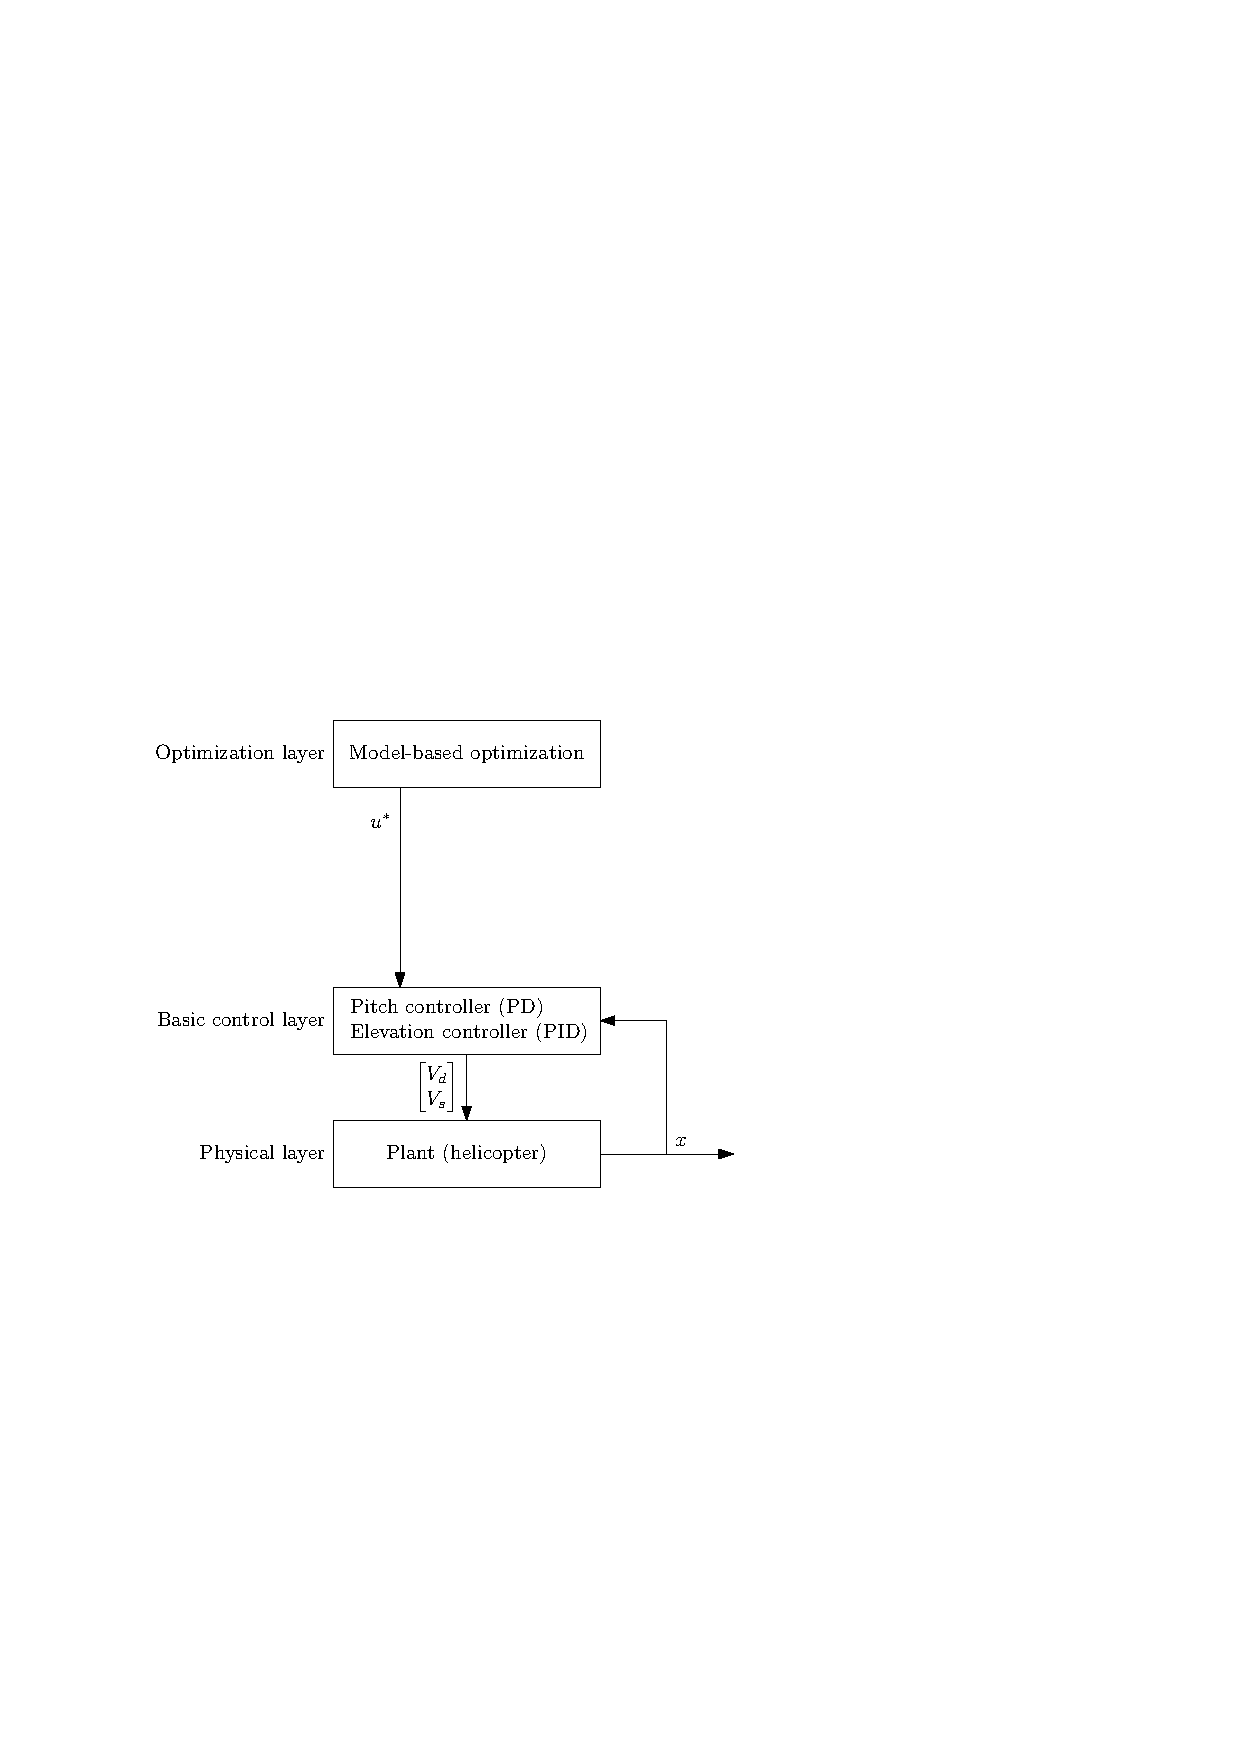
\includegraphics[width=1.00\textwidth]{figures/layers_openloop.pdf}
	\caption{A figure created with Ipe for TTK4135.}
\label{fig:layers_openloop}
\end{figure}
